% A Machine-Checked Formalization of the Pumping Lemma for Context-Free
% Languages via Pushdown Automata -- LLNCS version.
%
\documentclass[runningheads]{llncs}
%
\usepackage[T1]{fontenc}
\usepackage{graphicx}
\usepackage{amsmath}
\usepackage{amssymb}
\usepackage{fancyvrb}
\usepackage{xcolor}
\usepackage{tikz}
\usepackage{hyperref}
\renewcommand\UrlFont{\color{blue}\rmfamily}
\urlstyle{rm}

%% -- Colour helpers ----------------------------------------------------------
\newcommand{\blueFG}[1]{\textcolor[rgb]{0,0,0.8}{#1}}
\newcommand{\redFG}[1]{\textcolor[rgb]{0.6,0,0}{#1}}
\newcommand{\greenFG}[1]{\textcolor[rgb]{0,0.4,0}{#1}}
\newcommand{\purpleFG}[1]{\textcolor[rgb]{0.4,0,0.4}{#1}}

%% -- Semantic markup ---------------------------------------------------------
\newcommand{\D}[1]{{\blueFG{\textsf{#1}}}}      % datatype / type constructor
\newcommand{\Con}[1]{{\redFG{\textsf{#1}}}}     % data constructor
\newcommand{\F}[1]{{\greenFG{\textsf{#1}}}}     % function / definition
\newcommand{\V}[1]{{\purpleFG{\textit{#1}}}}    % variable / parameter
\newcommand{\Kw}[1]{\textbf{#1}}                % keyword

%% -- Links to the formalization ----------------------------------------------
%% \agdarev is the revision the links point to; it is set to the release tag
%% of the artifact accompanying this paper.
\newcommand{\agdarev}{main}
\newcommand{\agdarepo}{https://github.com/lives-group/pda-pumping/blob/\agdarev/src}
%% \agdalink{file}{line}{identifier}
\newcommand{\agdalink}[3]{\href{\agdarepo/#1\#L#2}{\F{#3}}}

%% -- Math-in-text helpers ----------------------------------------------------
\newcommand{\kto}{\ensuremath{\to}}
\newcommand{\kuplus}{\ensuremath{\uplus}}
\newcommand{\kfa}{\ensuremath{\forall}}
\newcommand{\kin}{\ensuremath{\in}}
\newcommand{\keq}{\ensuremath{\equiv}}
\newcommand{\kpda}{\ensuremath{\vdash_{\mathsf{p}}}}
\newcommand{\kpRa}{\ensuremath{\Longrightarrow}}
\newcommand{\kpRas}{\ensuremath{\Longrightarrow^{*}}}
\newcommand{\ks}[1]{\ensuremath{_{#1}}}
\newcommand{\kp}[1]{\ensuremath{^{#1}}}
\newcommand{\kla}{\ensuremath{\lambda}}
\newcommand{\kSigma}{\ensuremath{\Sigma}}
\newcommand{\kb}{\ensuremath{\beta}}
\newcommand{\kG}{\ensuremath{\Gamma}}   % stack ALPHABET
\newcommand{\kg}{\ensuremath{\gamma}}   % a stack (string of stack symbols)
\newcommand{\kd}{\ensuremath{\delta}}
\newcommand{\knat}{\ensuremath{\mathbb{N}}}
\newcommand{\ktimes}{\ensuremath{\times}}
\newcommand{\kle}{\ensuremath{\le}}
\newcommand{\klt}{\ensuremath{<}}
\newcommand{\kmaybe}{\ensuremath{\mathsf{Maybe}}}

%% -- Code block --------------------------------------------------------------
\DefineVerbatimEnvironment{spec}{Verbatim}%
{fontsize=\small,commandchars=\\\{\},xleftmargin=1em,
frame=none,samepage=true}

\begin{document}
%
\title{A Machine-Checked Formalization of the Pumping
Lemma for Context-Free Languages via Pushdown Automata}
%
\titlerunning{Formalizing the Pumping Lemma via Pushdown Automata}
%
\author{Rodrigo Ribeiro\orcidID{0000-0003-0131-5234}}
%
\authorrunning{R. Ribeiro}
%
\institute{Departamento de Computa\c{c}\~{a}o, Universidade Federal
  de Ouro Preto,
  Ouro Preto, MG, Brazil \\
\email{rodrigo.ribeiro@ufop.edu.br}}
%
\maketitle
%
\begin{abstract}
  We present a machine-checked formalization, in the dependently typed language
  Agda, of the pumping lemma for context-free languages, proved through pushdown
  automata instead of parse trees. The lemma says that every sufficiently long
  word $w$ of the language splits as $w = u\,v\,x\,y\,z$, with $v\,y$ non-empty
  and $v\,x\,y$ short, such that every $u\,v^{k}x\,y^{k}z$ is in the language.
  In our proof, the factors $v$ and $y$ are the input read by two segments of an
  accepting computation that return the stack to the same configuration, so that
  they can be repeated or removed. The theorem is stated about an
  \emph{arbitrary} pushdown automaton and its empty-stack language; grammars are
  never mentioned. Three ingredients are central: a normalization procedure that
  makes every step change the stack height by one while preserving the whole
  language, the empty word included; a well-founded recursion on the length of
  the computation that secures a non-empty pumped factor; and a search over the
  nested sub-computations of the run that bounds $|v\,x\,y|$. As an application,
  we prove in Agda that $\{a^{n}b^{n}c^{n}\}$ is not accepted by any pushdown
  automaton.

\keywords{Pumping lemma \and Pushdown automata \and Context-free
  languages \and Formal verification \and Agda \and Dependent types.}
\end{abstract}
%
%%---------------------------------------------------------------------------
\section{Introduction}\label{sec:intro}
%%---------------------------------------------------------------------------

The pumping lemma for context-free languages (CFLs) is the standard tool for
proving a language \emph{not} context-free. It says that every CFL $L$ has a
constant $p$ such that any word $w \in L$ with $|w| > p$ factors as
$w = u\,v\,x\,y\,z$ with $|v\,y| \geq 1$, $|v\,x\,y| \leq p$, and
$u\,v^{k}\,x\,y^{k}\,z \in L$ for every $k \geq 0$. The textbook
proof~\cite{hopcroft06,sipser13}, due to Bar-Hillel, Perles, and
Shamir~\cite{BarHillel61}, fixes a grammar in Chomsky Normal Form and argues on
parse trees: a tall enough tree has a root-to-leaf path repeating a
non-terminal, and the subtree at the repetition is what pumps. Amarilli and
Jeanmougin~\cite{Amarilli12} gave an alternative, informal proof through
\emph{pushdown automata} (PDAs), which never builds a tree; this paper
mechanizes that route.

The PDA proof argues about the \emph{stack profile} of an accepting
computation: the sequence of stack heights along the run. In a PDA whose every
step pushes or pops exactly one symbol, the profile is a path of integers that
moves by $\pm 1$, starting at $1$ and ending at $0$. Two situations then produce
pumpable segments (Fig.~\ref{fig:profile}). If the stack stays low, the run has
more positions than there are configurations of bounded height, so some
configuration (state and whole stack) occurs twice, and the segment between the
two occurrences is a loop that can be repeated or deleted. If the stack climbs
high, we look at the levels crossed on the way up to the peak and on the way
back down: two levels $g < h$ are entered and left in the same states with the
same top symbol, so the ascent from $g$ to $h$ and the descent from $h$ to $g$
can be repeated \emph{together}, giving the two factors $v$ and $y$. Both
situations are stated purely in terms of stacks and computations.

\paragraph{Motivation.}
A mechanization of the classical route already exists~\cite{RamosPumping16}, so
it is fair to ask what a second one adds. Three things. First, the statement:
ours is about the language of a bare automaton, so a user who models a system as
a PDA (as is common in interprocedural program analysis and model checking of
recursive programs~\cite{Reps98,AlurMadhusudan04}) can apply it without first
converting the automaton to a grammar. Second, the content: the proof is
constructive, so each witness (the pumping length, the five factors, and, for
every $k$, an accepting computation of the pumped word) is a value computed by
an Agda function, and the development has no postulates. Third, the reuse: the
geometry of stack profiles does not mention pumping, and is the natural basis for
the PDA proofs of Ogden's lemma and of related iteration properties. Making the
informal PDA argument fully precise also exposed two points that it glosses
over, the non-emptiness of $v\,y$ and the treatment of the empty word, both
discussed below.

\paragraph{Scope.}
We prove the lemma for the empty-stack language $L(M)$ of an arbitrary PDA $M$
over finite alphabets. That every CFL is the empty-stack language of some PDA is
the classical grammar-to-PDA construction~\cite{hopcroft06}; we do \emph{not}
formalize it here, so our theorem is the pumping lemma for CFLs exactly up to
that standard equivalence. Its formalization is future work
(Section~\ref{sec:conclusion}).

\paragraph{Contributions.}
\begin{itemize}
\item A direct PDA-to-PDA normalization turning an arbitrary automaton into one
  whose every step changes the stack height by $\pm 1$, preserving the full
  language, $\varepsilon$ included (Section~\ref{sec:normalization}).
\item A formalization of the geometry of stack profiles: a discrete
  intermediate-value theorem, the last and first passes through a level, and a
  pigeonhole over \emph{surface configurations} (Section~\ref{sec:geometry}).
\item The pumping lemma with all its conditions, $|v\,y| \geq 1$ and
  $|v\,x\,y| \leq p$ included, for an arbitrary PDA, with total functions
  rebuilding every pumped computation (Section~\ref{sec:pipeline}), and its use
  to prove that $\{a^{n}b^{n}c^{n}\}$ is not a PDA language
  (Section~\ref{sec:application}).
\end{itemize}

Section~\ref{sec:setup} introduces Agda and pushdown automata.
Section~\ref{sec:overview} gives the informal proof that the formalization
follows. Sections~\ref{sec:normalization} to~\ref{sec:pipeline} formalize its
three parts: normalization, the geometry of stack profiles, and the
reconstruction of pumped computations. Section~\ref{sec:application} applies the
lemma, Section~\ref{sec:related} discusses related work and
Section~\ref{sec:conclusion} concludes.

\paragraph{Artifact.}
The development uses Agda 2.7.0.1 and standard library 2.2; it is
available online~\cite{repo}, with a Nix build that type-checks it. Every module
is checked with the \texttt{--safe} flag, which rules out postulates and other
unsafe features, and the module \texttt{Everything.agda} imports every result
stated in this paper. Each theorem and lemma below is labelled with the Agda
identifier that proves it, as a hyperlink to its definition, and
Appendix~\ref{app:map} lists them all together with the full Agda types of the
main theorems. We show the main definitions and statements; the proofs,
which are long pattern-matching functions, are summarized in
Appendix~\ref{app:proofs}.

%%---------------------------------------------------------------------------
\section{Background}\label{sec:setup}
%%---------------------------------------------------------------------------

\subsection{Agda}

Agda is a dependently typed functional language based on Martin-L\"{o}f type
theory~\cite{Lof84}. Through the Curry-Howard correspondence~\cite{Howard80}
its types are propositions and its programs are proofs: to prove a theorem is to
write a total function of the type that states it, and an appeal to the
induction hypothesis is a recursive call. A small example illustrates the
notation. Lists form an inductive type, and that the empty list is a right unit
of concatenation is proved by induction on the left list, i.e., by a recursive
function into the equality type $\keq$:
\begin{spec}
\Kw{data} \D{List} (\V{A} : \D{Set}) : \D{Set} \Kw{where}
   \Con{[]}   : \D{List} \V{A}
   \Con{\_::\_} : \V{A} \kto{} \D{List} \V{A} \kto{} \D{List} \V{A}

\F{++-idr} : (\V{xs} : \D{List} \V{A}) \kto{} \V{xs} \F{++} \Con{[]} \keq{} \V{xs}
\F{++-idr} \Con{[]} = \Con{refl}
\F{++-idr} (\V{x} :: \V{xs}) = \F{cong} (\V{x} ::\_) (\F{++-idr} \V{xs})
\end{spec}
The type $\D{Maybe}\;\V{A}$ has constructors $\Con{nothing}$ and
$\Con{just}\;\V{a}$. The dependent pair $\kSigma$ (written $\exists$ when the
first component's type is inferable) is the existential quantifier, and the
disjoint sum $\kuplus$, with injections $\Con{inj\ks{1}}$ and
$\Con{inj\ks{2}}$, is disjunction. Recursions that do not decrease structurally
are justified by the accessibility predicate \D{Acc} of the standard library: a
function that matches on a certificate $\Con{acc}\;\V{rs}$ may call itself on any
$y$ below $x$, using the certificate $\V{rs}\;\V{p}$ obtained from a proof
$\V{p}$ that $y < x$. We use it with \F{<-wellFounded} on the natural numbers,
taking the \emph{length of a computation} as the measure. We refer
to~\cite{Wadler22} for a fuller account of Agda.

\subsection{Pushdown Automata and Acceptance}\label{sec:pda}

We fix types $Q$, $T$, and $\kG$ of states, input symbols, and stack symbols. A
pushdown automaton is a record with a transition function, an initial state,
and an initial stack symbol (\agdalink{PDA/Base.agda}{21}{PDA}):
\begin{spec}
\Kw{record} \D{PDA} (\V{Q} \V{T} \V{\kG{}} : \D{Set}) : \D{Set} \Kw{where}
   \Kw{field}
      \F{\kd{}} : \V{Q} \kto{} \D{Maybe} \V{T} \kto{} \V{\kG{}} \kto{} \D{List} (\V{Q} \ktimes{} \D{List} \V{\kG{}})
      \F{q\ks{0}} : \V{Q}
      \F{z\ks{0}} : \V{\kG{}}
\end{spec}
There are no final states: we only consider acceptance by empty stack. The
transition function takes a state, an \emph{optional} input symbol
(\Con{nothing} marks an $\varepsilon$-move) and the top stack symbol, and
returns the alternatives, each a target state paired with the string $\beta$
that replaces the popped top. A configuration is a triple of state, remaining
input, and stack ($\kg$ ranges over stacks, i.e., lists of stack symbols). One
step, and the multi-step closure, are:
\begin{spec}
\Kw{data} \D{\_\kpda{}\_\kpRa{}\_} (\V{M} : \D{PDA} \V{Q} \V{T} \V{\kG{}}) : \D{Config} \kto{} \D{Config} \kto{} \D{Set} \Kw{where}
   \Con{read} : (\V{r} , \V{\kb{}}) \kin{} \V{M} \F{.\kd{}} \V{q} (\Con{just} \V{a}) \V{A} \kto{}
          \V{M} \kpda{} (\V{q} , \V{a} :: \V{w} , \V{A} :: \V{\kg{}}) \kpRa{} (\V{r} , \V{w} , \V{\kb{}} ++ \V{\kg{}})
   \Con{eps}  : (\V{r} , \V{\kb{}}) \kin{} \V{M} \F{.\kd{}} \V{q} \Con{nothing}  \V{A} \kto{}
          \V{M} \kpda{} (\V{q} , \V{w} , \V{A} :: \V{\kg{}}) \kpRa{} (\V{r} , \V{w} , \V{\kb{}} ++ \V{\kg{}})

\Kw{data} \D{\_\kpda{}\_\kpRas{}\_} (\V{M} : \D{PDA} \V{Q} \V{T} \V{\kG{}}) : \D{Config} \kto{} \D{Config} \kto{} \D{Set} \Kw{where}
   \Con{\ensuremath{\varepsilon}}   : \V{M} \kpda{} \V{c} \kpRas{} \V{c}
   \Con{\_\ensuremath{\triangleleft}\_} : \V{M} \kpda{} \V{c\ks{1}} \kpRa{} \V{c\ks{2}} \kto{} \V{M} \kpda{} \V{c\ks{2}} \kpRas{} \V{c\ks{3}} \kto{} \V{M} \kpda{} \V{c\ks{1}} \kpRas{} \V{c\ks{3}}
\end{spec}
A computation is thus either empty ($\Con{\ensuremath{\varepsilon}}$) or a step
followed by a computation ($\_\Con{\ensuremath{\triangleleft}}\_$); \F{compLen}
counts its steps and \F{consumed} the input it reads. A word is accepted
\emph{by empty stack} when, from $\F{q}_0$ with $\F{z}_0$ alone on the stack, the
automaton can read all of it and empty its stack, in any state
(\agdalink{PDA/Language.agda}{15}{AccES}):
\begin{spec}
\F{AccES} : \D{PDA} \V{Q} \V{T} \V{\kG{}} \kto{} \D{List} \V{T} \kto{} \D{Set}
\F{AccES} \V{M} \V{w} = \D{\kSigma{}} \kla{} (\V{q} : \V{Q}) \kto{} \V{M} \kpda{} (\V{M} \F{.q\ks{0}} , \V{w} , \V{M} \F{.z\ks{0}} :: []) \kpRas{} (\V{q} , [] , [])
\end{spec}
We write $L(M) = \{\,w \mid \F{AccES}\;M\;w\,\}$ for the language of $M$.

%%---------------------------------------------------------------------------
\section{Overview of the Proof}\label{sec:overview}
%%---------------------------------------------------------------------------

\begin{figure}[t]
\centering
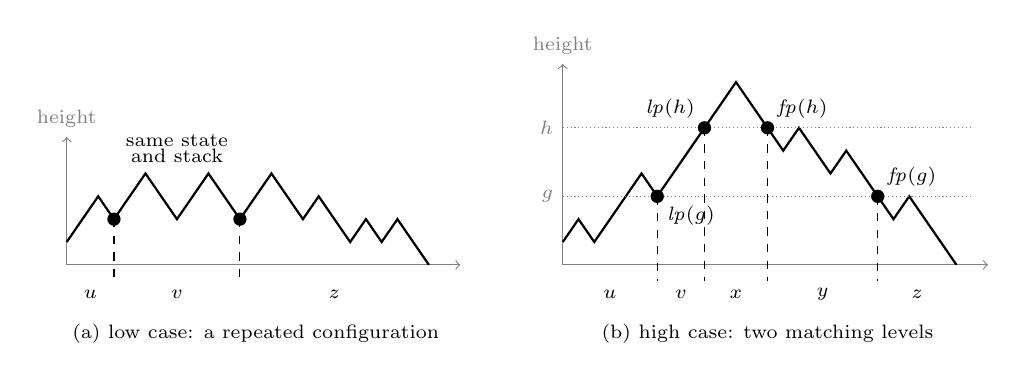
\begin{tikzpicture}[x=0.2cm,y=0.29cm,font=\scriptsize]
  % ---- low case -------------------------------------------------------------
  \begin{scope}
    \draw[->,gray] (0,0) -- (25,0);
    \draw[->,gray] (0,0) -- (0,5.6) node[above] {height};
    \draw[thick] (0,1) -- (1,2) -- (2,3) -- (3,2) -- (4,3) -- (5,4) -- (6,3)
      -- (7,2) -- (8,3) -- (9,4) -- (10,3) -- (11,2) -- (12,3) -- (13,4)
      -- (14,3) -- (15,2) -- (16,3) -- (17,2) -- (18,1) -- (19,2) -- (20,1)
      -- (21,2) -- (22,1) -- (23,0);
    \fill (3,2) circle (2.4pt); \fill (11,2) circle (2.4pt);
    \draw[dashed] (3,2) -- (3,-0.7); \draw[dashed] (11,2) -- (11,-0.7);
    \node at (1.5,-1.3) {$u$}; \node at (7,-1.3) {$v$}; \node at (17,-1.3) {$z$};
    \node[align=center] at (7,5.1) {same state\\[-2pt] and stack};
    \node at (12,-3) {(a) low case: a repeated configuration};
  \end{scope}
  % ---- high case ------------------------------------------------------------
  \begin{scope}[xshift=6.3cm]
    \draw[->,gray] (0,0) -- (27,0);
    \draw[->,gray] (0,0) -- (0,8.8) node[above] {height};
    \draw[thick] (0,1) -- (1,2) -- (2,1) -- (3,2) -- (4,3) -- (5,4) -- (6,3)
      -- (7,4) -- (8,5) -- (9,6) -- (10,7) -- (11,8) -- (12,7) -- (13,6)
      -- (14,5) -- (15,6) -- (16,5) -- (17,4) -- (18,5) -- (19,4) -- (20,3)
      -- (21,2) -- (22,3) -- (23,2) -- (24,1) -- (25,0);
    \draw[gray,densely dotted] (0,3) node[left] {$g$} -- (26,3);
    \draw[gray,densely dotted] (0,6) node[left] {$h$} -- (26,6);
    \foreach \p/\hh in {6/3,9/6,13/6,20/3} {
      \fill (\p,\hh) circle (2.4pt); \draw[dashed] (\p,\hh) -- (\p,-0.7); }
    \node[below right] at (6,3) {$\mathit{lp}(g)$};
    \node[above left] at (9,6) {$\mathit{lp}(h)$};
    \node[above right] at (13,6) {$\mathit{fp}(h)$};
    \node[above right] at (20,3) {$\mathit{fp}(g)$};
    \node at (3,-1.3) {$u$}; \node at (7.5,-1.3) {$v$}; \node at (11,-1.3) {$x$};
    \node at (16.5,-1.3) {$y$}; \node at (22.5,-1.3) {$z$};
    \node at (13,-3) {(b) high case: two matching levels};
  \end{scope}
\end{tikzpicture}
\caption{Stack profiles (stack height against position) of accepting
computations of a normal PDA, and the factors of the input read by each segment. In (b), $\mathit{lp}(g)$ is the last
position before the peak at height $g$ and $\mathit{fp}(g)$ the first after it;
the levels $g$ and $h$ have the same surface configuration.}
\label{fig:profile}
\end{figure}

This section gives the proof informally, with enough precision to follow the
formal development; the later sections formalize each step. Let $M$ be a PDA
over finite $Q$, $T$, $\kG$.

\paragraph{Step 1: normalize.} Build an automaton $M'$ with $L(M') = L(M)$ that
is \emph{normal}: every step either pops the top symbol or pushes one symbol on
top of it (Section~\ref{sec:normalization}). From now on we work with $M'$, and
transport the result back to $M$ at the end.

\paragraph{Step 2: the stack profile.} Let $d$ be an accepting computation of
$w$, of length $m$, and let $h_i$ be the stack height at position
$i \in [0,m]$. Then $h_0 = 1$, $h_m = 0$ and $|h_{i+1} - h_i| = 1$. Two facts
follow (Section~\ref{sec:geometry}). Since the profile moves by one, it cannot
skip a height (a discrete intermediate-value theorem). And since a push never
touches the symbols below the top, a segment of the run that never goes below
its starting height $h$ leaves the bottom $h$ symbols of the stack untouched; in
particular, two positions of equal height with nothing lower in between have the
\emph{same} stack.

\paragraph{Step 3: two cases.} Let $B$ be the peak of the profile and
$P = |Q|^{2}\cdot|\kG|$.
\begin{itemize}
\item \emph{Low case, $B \leq P+1$} (Fig.~\ref{fig:profile}(a)). Every
  configuration of $d$ is a state with a stack of height at most $P+1$; there
  are at most $N_0 = |Q|\cdot(|\kG|+1)^{P+1}$ of them. If $|w| > N_0$, then
  $d$, which reads one symbol per step at most, has more than $N_0$ positions, so
  a configuration repeats. The segment between the repetitions is a loop: it reads
  some $v$ and returns to the very same configuration, so it can be run $k$ times,
  or not at all, giving accepting computations of $u\,v^{k}z$.
\item \emph{High case, $B > P+1$} (Fig.~\ref{fig:profile}(b)). For each level
  $g$ between the base and the peak, let $\mathit{lp}(g)$ be the last position
  at height $g$ before the peak and $\mathit{fp}(g)$ the first after it. The
  \emph{surface configuration} of $g$ is the triple (state at $\mathit{lp}(g)$,
  top symbol at $\mathit{lp}(g)$, state at $\mathit{fp}(g)$). There are only $P$
  such triples and more than $P$ levels, so two levels $g < h$ share it. The
  ascent from $\mathit{lp}(g)$ to $\mathit{lp}(h)$ reads $v$ and stacks a block
  $\alpha$ above the stack at $\mathit{lp}(g)$; the descent from
  $\mathit{fp}(h)$ to $\mathit{fp}(g)$ reads $y$ and removes exactly such a
  block. Running the ascent $k$ times stacks $k$ blocks, the middle segment
  (reading $x$) runs on top of them unchanged, and $k$ descents remove them: this
  gives accepting computations of $u\,v^{k}x\,y^{k}z$.
\end{itemize}

\paragraph{Step 4: a non-empty factor.} In a normal PDA a loop may consist only
of $\varepsilon$-moves, so $v\,y$ may be empty. In that case we do not pump:
deleting the loop (the case $k=0$) gives a \emph{strictly shorter} accepting
computation of the same $w$, and we start again from it. Since computation
length is a natural number, after finitely many rounds the loop found reads at
least one symbol (Section~\ref{sec:vy}).

\paragraph{Step 5: bounding $|v\,x\,y|$.} Steps 3--4 give $v$, $x$ and $y$
without bound on their length. To bound them, we apply Steps 3--4 not to $d$ but
to a well-chosen \emph{excursion} of $d$: a segment that starts with some symbol
$A$ on top of the stack and ends when $A$ is popped. An excursion consists of
blocks, each a push followed by a smaller excursion (a \emph{child}), and a
final pop. We descend into a child as long as some child reads more than $N_0$
symbols. When none does, either the excursion has at most $|Q|$ blocks, so it
reads at most about $|Q|\cdot N_0$ symbols and Steps 3--4 applied to it yield a
short $v\,x\,y$, or it has more, and then two of its first $|Q|+1$ returns to the
base level occur in the same state, giving a short loop
(Section~\ref{sec:bounded}).

\paragraph{Constructive reading.} Read constructively, the lemma is an object
to be built. From $M$ the development computes a number $p$; and, for every word
$w$ accepted by $M$ with $p < |w|$, it computes the split of $w$ into five
factors, proofs that $v$ and $y$ are not both empty and that $|v\,x\,y| \leq p$,
and, for every $k$, an accepting computation of $u\,v^{k}\,x\,y^{k}\,z$. None of
these is a mere existence claim: each is a value that an Agda function computes
from the accepting computation it receives.

%%---------------------------------------------------------------------------
\section{Normalizing an Arbitrary Pushdown Automaton}\label{sec:normalization}
%%---------------------------------------------------------------------------

\subsection{The $\pm 1$ Normal Form}\label{sec:normal}

A PDA is \emph{normal} when every transition either pushes nothing, shrinking
the stack by one, or pushes a single new symbol on top of the restored old top,
growing it by one (\agdalink{PDA/Normal.agda}{24}{IsNormalPDA}):
\begin{spec}
\F{IsNormalPDA} : \D{PDA} \V{Q} \V{T} \V{\kG{}} \kto{} \D{Set}
\F{IsNormalPDA} \V{M} = \kfa{} \V{q} \V{mt} \V{A} \{\V{r}\} \{\V{\kb{}}\}
   \kto{} (\V{r} , \V{\kb{}}) \kin{} \V{M} \F{.\kd{}} \V{q} \V{mt} \V{A} \kto{} \V{\kb{}} \keq{} [] \kuplus{} \D{\kSigma{}} \kla{} \V{X} \kto{} \V{\kb{}} \keq{} \V{X} :: \V{A} :: []
\end{spec}
Abstracting away state and input, every step of a normal PDA is then a
\Con{pop} or a \Con{push} on the stack (lemma \F{normal-step}), and its effect on
the height is read off the indices
(\agdalink{PDA/Normal.agda}{78}{stackStep-\ensuremath{\pm}1}; Agda identifiers
may contain Unicode symbols such as $\pm$):
\begin{spec}
\Kw{data} \D{StackStep} : \D{List} \V{\kG{}} \kto{} \D{List} \V{\kG{}} \kto{} \D{Set} \Kw{where}
   \Con{pop}  : \D{StackStep} (\V{A} :: \V{\kg{}}) \V{\kg{}}
   \Con{push} : \D{StackStep} (\V{A} :: \V{\kg{}}) (\V{X} :: \V{A} :: \V{\kg{}})

\F{stackStep-\ensuremath{\pm}1} : \D{StackStep} \V{s} \V{s'}
   \kto{} (\F{length} \V{s} \keq{} \Con{suc} (\F{length} \V{s'})) \kuplus{} (\F{length} \V{s'} \keq{} \Con{suc} (\F{length} \V{s}))
\F{stackStep-\ensuremath{\pm}1} \Con{pop}  = \Con{inj\ks{1}} \Con{refl}
\F{stackStep-\ensuremath{\pm}1} \Con{push} = \Con{inj\ks{2}} \Con{refl}
\end{spec}
Both cases hold by computation, with no arithmetic to discharge. The indices of
\Con{push} also show that the tail $\kg$ is untouched, which is the invariant
suffix property of Step~2.

A stronger normal form, \D{IsNormalPDA\kp{+}}, also ties the polarity of a step
to whether it reads input: every read pops and every $\varepsilon$-move pushes.
It makes $|v\,y| \geq 1$ automatic, since a loop then reads as many symbols as it
performs $\varepsilon$-moves. But no such automaton accepts $\varepsilon$: to
empty a stack of height one, it must read one symbol more than it pushes. A
normalization that preserves the language of an automaton accepting
$\varepsilon$ must therefore target the weaker \F{IsNormalPDA}, which is why
Step~4 of the proof is needed. The development keeps the stronger variant as a
special case (Appendix~\ref{app:extra}).

\subsection{The Construction}\label{sec:construction}

Two obstacles separate an arbitrary $M$ from the normal form: a transition may
push a string $\beta$ of any length, and $M$ may empty its stack in ways the
discipline forbids. The construction, an adaptation of the textbook
transformations that bound the length of pushed strings~\cite{hopcroft06,Autebert97},
removes both by adding a bottom marker and bookkeeping states that push $\beta$
one symbol at a time.

Write $\bot$ for \Con{nothing} and $\widehat{A}$ for $\Con{just}\,A$. Let $\tau$
range over the transitions of $M$: a state $q$, an optional input symbol
$\mathit{mt}$, a top symbol $A$ and a choice of
$(r,\beta) \in \delta\,q\,\mathit{mt}\,A$; we write $\beta_\tau$ for its pushed
string. The normalized automaton $M'$ has
\[
\kG' = \kmaybe\,\kG,
\qquad
\F{z}_0' = \bot,
\qquad
Q' = \{\iota\}
   \cup \{\langle q\rangle\}_{q \in Q}
   \cup \{\langle \tau\rangle\}_{\tau}
   \cup \{\langle \tau,j\rangle\}_{1 \leq j < |\beta_\tau|},
\]
and encodes a stack $A_1 \cdots A_n$ of $M$ as
$\widehat{A_1} \cdots \widehat{A_n}\,\bot$. Its transitions, for every
transition $\tau$ of $M$ with $\beta_\tau = B_1 \cdots B_k$, are
\[
\begin{array}{r@{\;\ni\;}l@{\qquad}l}
\delta'(\iota, \varepsilon, \bot)
  & (\langle \F{q}_0\rangle,\; \widehat{\F{z}_0}\,\bot) & \\[2pt]
\delta'(\langle q\rangle, \mathit{mt}, \widehat{A})
  & (n_0,\; \varepsilon)
  & n_0 = \langle r\rangle \text{ if } k = 0, \text{ else } \langle \tau\rangle \\[2pt]
\delta'(\langle \tau\rangle, \varepsilon, C)
  & (n_k,\; \widehat{B_k}\,C)
  & n_k = \langle r\rangle \text{ if } k = 1, \text{ else } \langle \tau,k-1\rangle \\[2pt]
\delta'(\langle \tau,j\rangle, \varepsilon, C)
  & (n_j,\; \widehat{B_j}\,C)
  & n_j = \langle r\rangle \text{ if } j = 1, \text{ else } \langle \tau,j-1\rangle \\[2pt]
\delta'(\langle q\rangle, \varepsilon, \bot)
  & (\langle q\rangle,\; \varepsilon) &
\end{array}
\]
The first rule installs the encoded initial stack. The second pops the encoded
top symbol, reading an input symbol exactly when $\tau$ does, and passes control
to a push chain unless $\beta$ is empty. The third and fourth rules run that
chain, stacking $\beta$ in reverse so that $B_1$ ends on top, each step restoring
the symbol beneath. The last rule pops the marker, emptying the stack; this is
the step that lets $M'$ accept the empty word. Every rule is a legal pop or push,
so $M'$ is normal by construction, and $Q'$ is finite as soon as $Q$, $\kG$
\emph{and} $T$ are (since $\tau$ records the optional input symbol).

\begin{theorem}[\agdalink{PDA/NormalizePDA.agda}{566}{normalize}]\label{thm:normalize}
Let $M$ be a pushdown automaton over finite $Q$, $T$ and $\kG$. The automaton
$M'$ above is normal, its state type is finite, and $L(M') = L(M)$.
\end{theorem}

\noindent\emph{Proof sketch.} Normality and finiteness are read off the rules.
The equivalence is a simulation organized around the stack invariant: whenever
$M$ is in state $q$ with stack $s$, the simulation is in $\langle q\rangle$ with
$s$ encoded above the marker. Completeness ($L(M) \subseteq L(M')$) is by
induction on a computation of $M$, replacing each transition by its macro and
adding the marker push and pop; an $\varepsilon$-computation of $M$ becomes one
of $M'$, so the empty word is preserved. Soundness ($L(M') \subseteq L(M)$) is
by four mutually recursive functions that follow a computation of $M'$ and
reassemble each macro into the transition it simulates. Details are in
Appendix~\ref{app:proofs}. \qed

%%---------------------------------------------------------------------------
\section{The Geometry of Stack Profiles}\label{sec:geometry}
%%---------------------------------------------------------------------------

Fix a normal automaton $M$ and an accepting computation
$d : M \kpda{} (\F{q}_0 , w , \F{z}_0 :: []) \kpRas{} (q , [] , [])$ of length
$m = \F{compLen}\;d$. We write $\F{configAt}\;k\;d$ and $\F{stackAt}\;k\;d$ for
the configuration and stack after $k$ steps, and
$\F{s}_{\mathsf h}\,k\,d = \F{length}\,(\F{stackAt}\;k\;d)$ for the stack height.
These are projections of a function \F{splitAt} that cuts $d$ at position $k$
into a prefix and a suffix. The profile starts at $\F{s}_{\mathsf h}\,0\,d = 1$,
ends at $\F{s}_{\mathsf h}\,m\,d = 0$, and moves by one at each step, by
\F{stackStep-\ensuremath{\pm}1}.

\begin{lemma}[\agdalink{PDA/Pumping/IVT.agda}{25}{ivt}]\label{lem:ivt}
Let $a + n \leq m$. For every $h$ between $\F{s}_{\mathsf h}\,a\,d$ and
$\F{s}_{\mathsf h}\,(a+n)\,d$ (in either order), there is a position $p$ with
$a \leq p \leq a+n$ and $\F{s}_{\mathsf h}\,p\,d \equiv h$.
\end{lemma}

The proof is an induction on $n$ with a case analysis on the sign of each step;
it computes the witness $p$. The normalization of
Section~\ref{sec:normalization} is the hypothesis that makes the lemma true: for
an arbitrary PDA, whose steps may raise the stack by any amount, the profile can
skip heights. From \F{ivt} we obtain, for a height $h$ at or below the peak
position $j$, the \emph{last-pass} position $\F{lp}\;h \leq j$ at height $h$
(no later position up to $j$ has height $h$) and the \emph{first-pass} position
$\F{fp}\;h \geq j$ (no earlier position from $j$ on has height $h$).

\begin{lemma}[\agdalink{PDA/Pumping/LpFp.agda}{50}{stackAt-eq}]\label{lem:stackeq}
If $a \leq b \leq m$, the heights at $a$ and $b$ are equal, and no position in
$[a,b]$ has smaller height, then $\F{stackAt}\;a\;d \equiv \F{stackAt}\;b\;d$.
\end{lemma}

The extremality of \F{lp} and \F{fp} is exactly what makes this lemma
applicable: the profile stays at or above $g$ between $\F{lp}(g)$ and
$\F{fp}(g)$, and so the stacks at those two positions coincide, and likewise
for $h$. Let $B = \F{s}_{\mathsf h}\,j\,d$ be the peak, with $j$ computed by
\F{argmax}, and let
\[
P = |Q|^{2}\cdot|\kG|,
\qquad
\F{pumpLen} = |Q|\cdot(|\kG|+1)^{P+1},
\]
the latter being the number of pairs of a state and a stack of height at most
$P+1$. We write $|\mathrm{Cfg}_{\leq h}|$ for the number of such pairs with
stack height at most $h$, so that $\F{pumpLen} = |\mathrm{Cfg}_{\leq P+1}|$.
The two cases of Step~3 are separated by whether $B \leq P+1$. In the high case,
a pigeonhole over $Q \times \kG \times Q$
(\agdalink{PDA/Pumping/LpFp.agda}{409}{fullstate-collision}) yields two levels
$g < h$ with the same surface configuration.

%%---------------------------------------------------------------------------
\section{From Stack Profiles to the Pumping Lemma}\label{sec:pipeline}
%%---------------------------------------------------------------------------

Both cases rebuild pumped computations from loops with two pieces of surgery
from our trace library: \F{append-stack} replays a computation on top of extra
stack, by the invariant suffix property, and \F{swap-input} replays it with a
different passive input suffix, since a computation only reads the prefix it
consumes. With them, a segment that reads $v$ and returns to its starting
configuration can be repeated $k$ times (\F{loop-rep}), and a segment that reads
$v$ and grows the stack by a block can be run $k$ times stacking $k$ blocks.

\subsection{The Two Cases}\label{sec:low}\label{sec:high}

Each case is a function that, given an accepting computation $d$ of $w$ from a
one-symbol stack, returns \emph{either} a factorization that pumps \emph{or} a
strictly shorter accepting computation of the same $w$ with the same endpoints:
\begin{lemma}[\agdalink{PDA/Pumping/CaseLow.agda}{205}{caseLow-N},
  \agdalink{PDA/Pumping/CaseHigh.agda}{61}{caseHigh-N}]\label{lem:cases}
Let $M$ be normal and $d$ an accepting computation of $w$ with peak $B$.
\begin{itemize}
\item If $B \leq P+1$ and $\F{pumpLen} < |w|$, then either $w = u\,v\,z$ with
  $|v| \geq 1$ and $u\,v^{k}z \in L(M)$ for all $k$, or there is an accepting
  computation $d'$ of $w$ with $\F{compLen}\;d' < \F{compLen}\;d$.
\item If $B > P+1$, then either $w = u\,v\,x\,y\,z$ with $|v\,y| \geq 1$ and
  $u\,v^{k}x\,y^{k}z \in L(M)$ for all $k$, or there is such a $d'$.
\end{itemize}
\end{lemma}

In the low case, \F{find-loop} turns the configuration collision into a
factorization $d = d_1\,d_2\,d_3$ in which $d_2$ starts and ends in the same
state with the very same stack; $d_2$ can then be repeated or excised in place.
The hypothesis is stated at the actual peak $B$ and discharged from
$\F{pumpLen} < |w|$ by monotonicity of $|\mathrm{Cfg}_{\leq h}|$ in $h$. In the
high case, the four positions $\F{lp}(g)$, $\F{lp}(h)$, $\F{fp}(h)$, $\F{fp}(g)$
cut $d$ into the five segments of Fig.~\ref{fig:profile}(b), and two applications
of Lemma~\ref{lem:stackeq} give the stack equalities that make the loops
compatible. The function \F{double-pump} glues prefix, $k$ ascents, middle, $k$
descents and suffix into an accepting computation of $u\,v^{k}x\,y^{k}z$. The
synchronization is the delicate part: the $k$ ascents stack $k$ copies of a block
$X :: \alpha$, and the descents must remove exactly those copies, in order, after
the middle segment has run on top of them; this is the equation
$\F{rep}\;k\;(X :: \alpha) \mathbin{+\!+} X :: \gamma'$ between the stacks, where
$\F{rep}\;k\;t$ is $t$ repeated $k$ times. This construction is the most
expensive part of the development to type-check, and Appendix~\ref{app:extra}
describes how we keep that cost under control.

\subsection{A Non-Empty Pumped Factor}\label{sec:vy}

When the loop of the low case, or both loops of the high case, read no input,
each case returns its right disjunct: in the low case $d_1$ followed by $d_3$,
with the empty loop excised; in the high case the reconstruction for $k = 0$,
which skips both loops. Both are strictly shorter than $d$, since the loops have
at least one step, and both end in the same state as $d$. That the
reconstructions are shorter follows from lemmas stating that the surgery
operations preserve \F{compLen}.

This sets up a recursion: run the case analysis on $d$; if it returns a
factorization, we are done; if it returns a shorter computation $d'$ of the same
$w$, run it again on $d'$. The recursion terminates because \F{compLen} decreases
at each round, and it can only stop with a factorization, whose loop then reads
at least one symbol. Formally, a generic engine
(\agdalink{PDA/Pumping/PumpN.agda}{32}{pump-go}) takes the step function and an
\D{Acc} certificate for $\F{compLen}\;d$, and the recursive call on $d'$ uses the
certificate obtained from $\F{compLen}\;d' < \F{compLen}\;d$. The result is the
lemma without the bound on $|v\,x\,y|$
(\agdalink{PDA/Pumping/PumpNormal.agda}{75}{pda-pumping-N-at}), stated for any
computation from a one-symbol stack to the empty stack, with both endpoints
fixed.

\subsection{Bounding $|v\,x\,y|$}\label{sec:bounded}

The factors found so far may be long: in the low case $v$ may be preceded and
followed by arbitrarily long segments, but nothing bounds $v$ itself, and in the
high case nothing bounds $x$. We bound them by choosing \emph{where} to apply the
previous lemma.

An \emph{excursion} of a symbol $A$ is a computation from
$(q , w , A :: []) $ to $(q' , w' , [])$. Any accepting computation is an
excursion of $\F{z}_0$, and in a normal automaton every excursion decomposes
(\agdalink{PDA/Pumping/Excursion.agda}{146}{excView}): its first step either pops
$A$, and the excursion ends, or pushes some $X$ above $A$; in that case the run
continues with an excursion of $X$ over the floor $A :: []$ (the \emph{child},
which \agdalink{PDA/Pumping/Excursion.agda}{83}{firstReturn} cuts off at the
first moment the stack is $A :: []$ again) and then with the rest of the
excursion of $A$. An excursion is therefore a sequence of blocks, each a push
followed by a child, ended by a pop. Since the child never descends to the
floor, it can be run on its own and plugged back with \F{append-stack}, so
pumping a child yields a pumping of the whole computation, with the same factors
$v$, $x$, $y$.

Let $p_0 = \F{pumpLen}$ and set
\[
\F{pumpBound} = (|Q| + 1)\cdot(p_0 + 1).
\]
The search (\agdalink{PDA/Pumping/Bounded.agda}{405}{find}) takes an excursion
$e$ that reads more than $p_0$ symbols and proceeds as follows.
\begin{enumerate}
\item If $e$ reads at most \F{pumpBound} symbols, apply
  \F{pda-pumping-N-at} to $e$ itself: since $v\,x\,y$ is a factor of the input
  of $e$, $|v\,x\,y| \leq \F{pumpBound}$.
\item Otherwise, walk along the blocks of $e$
  (\agdalink{PDA/Pumping/Bounded.agda}{301}{walk}), recording, for each visit of
  the base level $A :: []$, its state. If a child reads more than $p_0$ symbols,
  search it recursively and plug the result back.
\item If a visit repeats the state of an earlier one, the blocks between them
  form a loop on an identical configuration (same state, stack $A :: []$),
  spanning at most $|Q|$ blocks, each reading at most $p_0 + 1$ symbols. If the
  loop reads something, it pumps with $x = y = \varepsilon$ and
  $|v| \leq |Q|\cdot(p_0+1)$. If it reads nothing, excise it and restart the
  search on the shorter excursion.
\item The walk cannot reach the final pop: all visits so far have distinct
  states, so there are at most $|Q|$ blocks, and $e$ would read at most
  $|Q|\cdot(p_0+1) + 1 \leq \F{pumpBound}$ symbols, contradicting case 1.
\end{enumerate}
The search recurses on children and on excised excursions, both strictly shorter
than $e$, so it is again justified by \D{Acc} on \F{compLen}; the walk along the
blocks is a nested well-founded recursion on the length of the remaining
excursion. Distinctness of the recorded states is tracked with the
\D{AllDistinct} predicate, whose length is bounded by $|Q|$ because $Q$ is
finite; decidable equality of states, needed to detect the repetition, follows
from finiteness by comparing positions in the listing of $Q$.

\begin{theorem}[\agdalink{PDA/Pumping/Arbitrary.agda}{31}{pda-pumping-N}]\label{thm:normal}
Let $M$ be a normal pushdown automaton over finite $Q$ and $\kG$, and
$p = \F{pumpBound}$. For every $w \in L(M)$ with $p < |w|$, there are
$u,v,x,y,z$ with $w = u\,v\,x\,y\,z$, $|v\,y| \geq 1$, $|v\,x\,y| \leq p$, and
$u\,v^{k}\,x\,y^{k}\,z \in L(M)$ for every $k$.
\end{theorem}

\subsection{The End-to-End Theorem}\label{sec:end}

Composing Theorem~\ref{thm:normalize} with Theorem~\ref{thm:normal} gives the
lemma for an arbitrary PDA. The constant is \F{pumpBound} computed from the
alphabets of the \emph{normalized} automaton. Because the normalization preserves
the language exactly, the empty word needs no separate handling, and every
pumped word is transported back through the equivalence. In Agda the statement
reads (\agdalink{PDA/Pumping/Arbitrary.agda}{52}{pumping-pda}):
\begin{spec}
\F{pumping-pda} : \F{Finite} \V{Q} \kto{} \F{Finite} \V{T} \kto{} \F{Finite} \V{\kG{}} \kto{} (\V{M} : \D{PDA} \V{Q} \V{T} \V{\kG{}})
  \kto{} \D{\kSigma{}} \kla{} (\V{p} : \knat{}) \kto{} \kfa{} \{\V{w}\} \kto{} \F{AccES} \V{M} \V{w} \kto{} \V{p} \klt{} \F{length} \V{w}
  \kto{} \D{\kSigma{}}[ \V{u} ] \D{\kSigma{}}[ \V{v} ] \D{\kSigma{}}[ \V{x} ] \D{\kSigma{}}[ \V{y} ] \D{\kSigma{}}[ \V{z} ] \V{w} \keq{} \V{u} ++ \V{v} ++ \V{x} ++ \V{y} ++ \V{z}
     \ktimes{} 0 \klt{} \F{length} \V{v} + \F{length} \V{y}
     \ktimes{} \F{length} (\V{v} ++ \V{x} ++ \V{y}) \kle{} \V{p}
     \ktimes{} (\kfa{} \V{k} \kto{} \F{AccES} \V{M} (\V{u} ++ \F{rep} \V{k} \V{v} ++ \V{x} ++ \F{rep} \V{k} \V{y} ++ \V{z}))
\end{spec}
\begin{theorem}[\agdalink{PDA/Pumping/Arbitrary.agda}{52}{pumping-pda}]\label{thm:end}
For every pushdown automaton $M$ over finite $Q$, $T$, and $\kG$, there is a
$p \in \knat$ such that every $w \in L(M)$ with $p < |w|$ factors as
$w = u\,v\,x\,y\,z$ with $|v\,y| \geq 1$, $|v\,x\,y| \leq p$, and
$u\,v^{k}\,x\,y^{k}\,z \in L(M)$ for every $k$.
\end{theorem}

\paragraph{The size of the pumping length.}
Normalization enlarges the automaton: $|\kG'| = |\kG| + 1$ and, in the Agda
encoding, $|Q'| = 1 + |Q| + |\Delta| + \sum_{\tau}|\beta_\tau|$, where $\Delta$
is the set of transitions of $M$. Since $P' = |Q'|^{2}\,(|\kG|+1)$ appears in an
exponent, the constant grows exponentially with the square of the size of
$\delta$, against the square of $|Q|$ if $M$ were already normal. For a
two-state PDA for $\{a^{n}b^{n}\}$ with two stack symbols and six transitions,
the constant computed from $M$ itself would be about $1.2 \cdot 10^{5}$, while
the one computed from $M'$ ($|Q'| = 13$) is about $10^{308}$. For comparison,
the textbook bound through grammars is also exponential, $2^{|V|}$ for a grammar
in Chomsky Normal Form with $|V|$ non-terminals, and the standard PDA-to-grammar
translation produces $|V| = |Q|^{2}\,|\kG|$ non-terminals. None of these bounds
is tight, and for applications of the lemma, which only use the existence of
$p$, their size is irrelevant.

%%---------------------------------------------------------------------------
\section{Application: $\{a^{n}b^{n}c^{n}\}$ is not a PDA Language}\label{sec:application}
%%---------------------------------------------------------------------------

The usual application of the lemma is to show that a language is not
context-free. We formalized the standard example, over the alphabet
$\D{\kSigma\ks{3}} = \{a,b,c\}$, with $\F{abc}\;n = a^{n}b^{n}c^{n}$ and
$\F{L-abc}\;w = \exists\,n.\; w \keq \F{abc}\;n$
(\agdalink{Examples/ABC.agda}{240}{abc-not-PDA}):
\begin{spec}
\F{abc-not-PDA} : \F{Finite} \V{Q} \kto{} \F{Finite} \V{\kG{}} \kto{} (\V{M} : \D{PDA} \V{Q} \D{\kSigma\ks{3}} \V{\kG{}})
  \kto{} \ensuremath{\neg} ((\kfa{} \V{w} \kto{} \F{AccES} \V{M} \V{w} \kto{} \F{L-abc} \V{w}) \ktimes{} (\kfa{} \V{w} \kto{} \F{L-abc} \V{w} \kto{} \F{AccES} \V{M} \V{w}))
\end{spec}
The proof follows the textbook argument. Let $p$ be given by
Theorem~\ref{thm:end} and take $w = a^{m}b^{m}c^{m}$ with $m = p+1$. Since
$|v\,x\,y| \leq p < m$, the factor $v\,x\,y$ cannot contain both an $a$ and a
$c$: if the prefix $u$ has length at least $m$, $v\,x\,y$ lies in
$b^{m}c^{m}$; otherwise $u\,v\,x\,y$ has length at most $2m$ and lies in
$a^{m}b^{m}$. Pumping down ($k = 0$) gives $u\,x\,z \in L(M)$, hence
$u\,x\,z = a^{n}b^{n}c^{n}$ for some $n$. It still has $m$ occurrences of the
letter that $v\,x\,y$ misses, so $n = m$, but it is shorter than $w$ by
$|v\,y| \geq 1$, a contradiction. The Agda proof counts letter occurrences with a
function that distributes over concatenation, and uses the ring solver of the
standard library for the arithmetic. One practical point: the proof must keep the
pumping length abstract, receiving $p$ and the pumping statement as arguments.
Unfolding the concrete $p$ produced by Theorem~\ref{thm:end}, a unary natural
number of the size discussed above, makes type-checking diverge in practice.

%%---------------------------------------------------------------------------
\section{Related work}\label{sec:related}
%%---------------------------------------------------------------------------

The proof we formalize is due to Amarilli and Jeanmougin~\cite{Amarilli12}.
Their account is informal; we make every step of the stack-profile geometry, the
two-case pigeonhole and the loop reconstructions explicit and machine-checked, and
we add three ingredients that the informal version does not spell out: the
language-exact normalization, the well-founded argument for $|v\,y| \geq 1$, and
the search over excursions that bounds $|v\,x\,y|$.

The theorem itself has been mechanized before. Ramos et
al.~\cite{RamosPumping16} formalize the context-free pumping lemma in Rocq by the
classical route, from a Chomsky Normal Form grammar and a long derivation tree,
within a larger library of context-free language theory, and later use it to
prove specific languages non-context-free and context-free languages not closed
under intersection~\cite{RamosApplications19}. Barthwal and
Norrish~\cite{Barthwal10,Barthwal10thesis} reach the same theorem in HOL4,
within a substantial fragment of context-free language theory, in a classical
setting where the witnessing functions are not extracted as programs. Our work
differs from both in what is proved and how. We argue on automata and never build
a tree, so the combinatorics is the geometry of a stack profile rather than the
branching of a derivation. Our statement quantifies over an arbitrary pushdown
automaton and mentions no grammar. And the proof is constructive. Comparing sizes
is less informative, since the developments cover different amounts of
surrounding theory; we only note that ours, about 4,600 lines including the
normalization and the example, is self-contained.

Mechanizations of the surrounding theory are more common. Firsov and
Uustalu~\cite{Firsov15} certify the conversion of grammars to Chomsky Normal Form
in Agda, and CYK parsing for such grammars~\cite{Firsov14}. Ramos et
al.~\cite{Ramos15} formalize grammar simplification, and
Dvo\v{r}\'{a}k and Blanchette~\cite{Dvorak23} verify closure properties of
general grammars in Lean. The recent Isabelle/HOL formalization of context-free
grammar theory by Nipkow et al.~\cite{NipkowLRY-IJCAR26} covers normal forms and
several deep theorems on the grammar side. The pumping lemma through pushdown
automata, with a language-exact PDA normal form, is to our knowledge not among
the existing machine-checked treatments.

On the regular side, Doczkal, Kaiser and Smolka~\cite{Doczkal13} develop a
constructive theory of regular languages in Rocq, the pumping lemma among its
results, in SSReflect, later extended to a systematic account of regular language
representations~\cite{DoczkalSmolka18}. Hobor, Li and Stephan~\cite{Hobor19}
formalize the pumping properties of Jaffe and of Ehrenfeucht, Parikh and
Rozenberg, and find that the classical proof that block cancellation implies
regularity appeals to the axiom of choice. We share their concern one level up in
the hierarchy: a constructive reading of a pumping statement has to produce its
witnesses, which is why the non-emptiness of the pumped factor costs a
well-founded recursion here instead of a counting argument. Certified parsing of
regular expressions~\cite{Lopes16,Cardoso23} shares our broader goal of a
verified language-theory library.

%% ---------------------------------------------------------------------------
\section{Conclusion}\label{sec:conclusion}
%%---------------------------------------------------------------------------

We presented a machine-checked Agda formalization of the pumping lemma for
context-free languages by the pushdown-automaton route, stated about the
empty-stack language of an arbitrary automaton, with all the conditions of
the lemma, $|v\,x\,y| \leq p$ included. Its core is a $\pm 1$ normal form, reached by a
language-exact normalization, whose stack profile admits a discrete
intermediate-value theorem and a pigeonhole over surface configurations; the
non-emptiness of $v\,y$ and the bound on $v\,x\,y$ are obtained by well-founded
searches over computations. The stack-profile layer does not mention pumping, so
it can be reused as it stands. As future work, we intend to use it for
\emph{Ogden's lemma} and for pumping downwards, already supported by the
shortening step of Section~\ref{sec:vy}, and to formalize the grammar-to-PDA
construction, which would turn Theorem~\ref{thm:end} into the grammar-level
statement.

\begin{credits}
\subsubsection{\ackname}
The author thanks the anonymous reviewers for their helpful comments.

\subsubsection{\discintname}
The author has no competing interests to declare that are relevant to the
content of this article.
\end{credits}

%%---------------------------------------------------------------------------
\bibliographystyle{splncs04}
\bibliography{references}

%%---------------------------------------------------------------------------
\newpage
\appendix
%%---------------------------------------------------------------------------
\section{Proofs}\label{app:proofs}
%%---------------------------------------------------------------------------

For the reader's convenience each statement is repeated before its proof. Except
in the first, $M$ is a normal automaton, $d$ an accepting computation of length
$m$, and $\F{s}_{\mathsf h}\,k\,d$ the stack height at position $k$.

\medskip
\noindent\textbf{Theorem~\ref{thm:normalize} (\F{normalize}).}
\emph{Let $M$ be a pushdown automaton over finite $Q$, $T$ and $\kG$. The
automaton $M'$ of Section~\ref{sec:construction} is normal, its state type is
finite, and $L(M') = L(M)$.}
\begin{proof}
Normality is read off the five rules: each is a pop, replacing the top symbol by
the empty string, or a push of one symbol above the restored top. Finiteness of
$Q'$ follows from that of $Q$, $\kG$ and $T$, since a transition $\tau$ is
determined by a state, an optional input symbol, a top symbol and an index into
the list $\delta$ returns for them.

The equivalence is a step-by-step simulation organized around the stack
invariant: whenever $M$ is in state $q$ with stack $s$, the simulation is in
$\langle q\rangle$ with $s$ encoded above the marker. Completeness
(\F{normalize-complete}) is by induction on a computation of $M$, replacing each
transition by its macro and the start and end by the marker push and pop; an
$\varepsilon$-computation of $M$ becomes an $\varepsilon$-computation of $M'$, so
the empty word is preserved. Soundness (\F{normalize-sound}) inverts each macro
by four mutually recursive functions that follow $M'$ structurally, using the
non-emptiness of the intermediate stacks to rule out spurious base cases; a stack
invariant on the push-slicing states $\langle\tau\rangle$ and
$\langle\tau,j\rangle$ tracks how far a macro has progressed. \qed
\end{proof}

\medskip
\noindent\textbf{Lemma~\ref{lem:stackeq} (\F{stackAt-eq}).}
\emph{If $a \leq b \leq m$, the heights at $a$ and $b$ are equal, and no position
in $[a,b]$ has smaller height, then
$\F{stackAt}\;a\;d \equiv \F{stackAt}\;b\;d$.}
\begin{proof}
The segment from $a$ to $b$ never descends below the common height, so the stack
present at $a$ is an invariant suffix throughout: by the push-preserves-tail
property of normal steps it is carried unchanged to $b$ as a suffix of
$\F{stackAt}\;b\;d$. Since the two stacks have the same length, the part above
the suffix is empty, and the stacks coincide. \qed
\end{proof}

\medskip
\noindent\textbf{Theorem~\ref{thm:normal} (\F{pda-pumping-N}).}
\emph{Let $M$ be a normal pushdown automaton over finite $Q$ and $\kG$, and
$p = \F{pumpBound}$. For every $w \in L(M)$ with $p < |w|$, there are
$u,v,x,y,z$ with $w = u\,v\,x\,y\,z$, $|v\,y| \geq 1$, $|v\,x\,y| \leq p$, and
$u\,v^{k}\,x\,y^{k}\,z \in L(M)$ for every $k$.}
\begin{proof}
First, \F{pda-pumping-N-at}: for any computation from
$(q, w, A :: [])$ to $(q_f, [], [])$ with $\F{pumpLen} < |w|$, there is a factorization with
$|v\,y| \geq 1$ whose pumped computations end in $q_f$. It is \F{pump-run} applied
to the step function that computes the peak with \F{argmax}, branches on
$B \leq P+1$, and calls \F{caseLow-N} (taking $x = y = \varepsilon$, after
rewriting $\F{rep}\;k\;[] = []$) or \F{caseHigh-N}. Termination is the
well-founded recursion on \F{compLen}; at every leaf the loop found consumes
input, so $|v\,y| \geq 1$.

Then \F{find}, by well-founded recursion on \F{compLen}, for an excursion $e$
reading more than $p_0 = \F{pumpLen}$ symbols. If $e$ reads at most $p$ symbols,
apply \F{pda-pumping-N-at} to $e$, made input-exact by \F{exact}; the bound
follows since $v\,x\,y$ is a factor of the input of $e$. Otherwise \F{walk}
traverses the blocks of $e$ with \F{excView}, maintaining the prefix
\textsf{PRE} of $e$ up to the current visit of the base level, the number $n$ of
blocks traversed, the bound $|\F{consumed}\;\textsf{PRE}| \leq n\,(p_0+1)$, and
a list of the earlier visits in pairwise distinct states, each with the segment
from it to the current visit, reading at most $n\,(p_0+1)$ symbols. Distinctness
gives $n \leq |Q|$. If the current state occurs in the list, \F{repeat} either
pumps the segment with $x = y = \varepsilon$ (\F{loopPump}) or, if it reads
nothing, excises it and calls \F{find} on the shorter excursion
(\F{shortcut}). Otherwise \F{excView} exposes the next step. A pop would make
$e$ read at most $|Q|\,(p_0+1)+1 \leq p$ symbols, a contradiction. A push
followed by a child $c$: if $c$ reads more than $p_0$ symbols, \F{find} is called
on $c$ and its result transported to $e$ (\F{embed}, using \F{append-stack},
\F{extend-input} and \F{swap-input}); otherwise the block reads at most $p_0 + 1$
symbols and the walk continues. Finally, \F{bounded-pumping} applies \F{find} to
an accepting computation, and \F{pda-pumping-N} repackages the result. \qed
\end{proof}

\medskip
\noindent\textbf{Theorem~\ref{thm:end} (\F{pumping-pda}).}
\emph{For every pushdown automaton $M$ over finite $Q$, $T$, and $\kG$, there
is a $p \in \knat$ such that every $w \in L(M)$ with $p < |w|$ factors as
$w = u\,v\,x\,y\,z$ with $|v\,y| \geq 1$, $|v\,x\,y| \leq p$, and
$u\,v^{k}\,x\,y^{k}\,z \in L(M)$ for every $k$.}
\begin{proof}
Normalize $M$ to $M'$, with the language equivalence and the finiteness of its
state and stack alphabets. Take $p = \F{pumpBound}$ computed from those sizes.
Given $w \in L(M)$ with $p < |w|$, transport it to $w \in L(M')$ by
completeness, apply Theorem~\ref{thm:normal}, and transport each pumped word back
to $M$ by soundness. \qed
\end{proof}

%%---------------------------------------------------------------------------
\section{Implementation Notes}\label{app:extra}
%%---------------------------------------------------------------------------

\paragraph{The strong normal form.} The development also contains the stronger
normal form
\begin{spec}
\Kw{record} \D{IsNormalPDA\kp{+}} (\V{M} : \D{PDA} \V{Q} \V{T} \V{\kG{}}) : \D{Set} \Kw{where}
   \Kw{field}
      \F{read-pops}  : (\V{r} , \V{\kb{}}) \kin{} \V{M} \F{.\kd{}} \V{q} (\Con{just} \V{a}) \V{A} \kto{} \V{\kb{}} \keq{} []
      \F{eps-pushes} : (\V{r} , \V{\kb{}}) \kin{} \V{M} \F{.\kd{}} \V{q} \Con{nothing} \V{A} \kto{}
                  \D{\kSigma{}} \kla{} \V{X} \kto{} \V{\kb{}} \keq{} \V{X} :: \V{A} :: []
\end{spec}
which implies \F{IsNormalPDA}. For it, the theorem \F{pda-pumping}
(\agdalink{PDA/Pumping/Lemma.agda}{76}{pda-pumping}) obtains $|v\,y| \geq 1$
directly by the counting argument \F{balance}: initial height plus number of
$\varepsilon$-moves equals final height plus number of reads, so a loop, whose
endpoints have equal height, reads as many symbols as it performs
$\varepsilon$-moves. Both theorems share the geometric core: the high-case
reconstruction is carried out once, under the weaker hypothesis, and returns the
proof of $|v\,y| \geq 1$ as a function still expecting an
\D{IsNormalPDA\kp{+}} witness, which the arbitrary-automaton path never applies.

\paragraph{Opaque definitions.} To decide whether two types are equal, Agda
normalizes terms, unfolding definitions. The high-case reconstruction returns
its witnesses inside a record whose construction has a large normal form, while
its consumers only depend on its type. We place the function that builds it in
an \Kw{opaque} block: outside the block Agda sees only its type, so modules
downstream do not rebuild the construction just to read one field. Inside, the
definition computes as usual, and an \Kw{unfolding} declaration can expose it at
a chosen site. Similarly, we consume the large sum types returned by the case
functions by function application rather than by \Kw{with}-abstraction, which in
contexts with many free variables generalizes every pending goal over the whole
telescope and exhausts memory.

%%---------------------------------------------------------------------------
\section{Correspondence with the Formalization}\label{app:map}
%%---------------------------------------------------------------------------

Table~\ref{tab:map} lists, for each result of the paper, the Agda identifier that
proves it and its module; the identifiers are hyperlinks to the definitions in
the artifact~\cite{repo}. The module \texttt{Everything.agda} imports all of them.

\begin{table}[h]
\centering
\caption{Results of the paper and their Agda counterparts (modules under
\texttt{src/}).}\label{tab:map}
\begin{tabular}{lll}
\hline
Result & Agda identifier & Module \\
\hline
PDA, acceptance & \agdalink{PDA/Base.agda}{21}{PDA}, \agdalink{PDA/Language.agda}{15}{AccES} & \texttt{PDA/Base}, \texttt{PDA/Language} \\
Normal form & \agdalink{PDA/Normal.agda}{24}{IsNormalPDA} & \texttt{PDA/Normal} \\
Theorem~\ref{thm:normalize} & \agdalink{PDA/NormalizePDA.agda}{566}{normalize} & \texttt{PDA/NormalizePDA} \\
Lemma~\ref{lem:ivt} & \agdalink{PDA/Pumping/IVT.agda}{25}{ivt} & \texttt{PDA/Pumping/IVT} \\
Lemma~\ref{lem:stackeq} & \agdalink{PDA/Pumping/LpFp.agda}{50}{stackAt-eq} & \texttt{PDA/Pumping/LpFp} \\
Surface pigeonhole & \agdalink{PDA/Pumping/LpFp.agda}{409}{fullstate-collision} & \texttt{PDA/Pumping/LpFp} \\
Lemma~\ref{lem:cases} & \agdalink{PDA/Pumping/CaseLow.agda}{205}{caseLow-N}, \agdalink{PDA/Pumping/CaseHigh.agda}{61}{caseHigh-N} & \texttt{PDA/Pumping/Case*} \\
Double pump & \agdalink{PDA/Pumping/CaseHighCore.agda}{92}{double-pump} & \texttt{PDA/Pumping/CaseHighCore} \\
Engine (Sect.~\ref{sec:vy}) & \agdalink{PDA/Pumping/PumpN.agda}{32}{pump-go} & \texttt{PDA/Pumping/PumpN} \\
Unbounded lemma & \agdalink{PDA/Pumping/PumpNormal.agda}{75}{pda-pumping-N-at} & \texttt{PDA/Pumping/PumpNormal} \\
Excursions & \agdalink{PDA/Pumping/Excursion.agda}{146}{excView} & \texttt{PDA/Pumping/Excursion} \\
Search (Sect.~\ref{sec:bounded}) & \agdalink{PDA/Pumping/Bounded.agda}{405}{find} & \texttt{PDA/Pumping/Bounded} \\
Theorem~\ref{thm:normal} & \agdalink{PDA/Pumping/Arbitrary.agda}{31}{pda-pumping-N} & \texttt{PDA/Pumping/Arbitrary} \\
Theorem~\ref{thm:end} & \agdalink{PDA/Pumping/Arbitrary.agda}{52}{pumping-pda} & \texttt{PDA/Pumping/Arbitrary} \\
Strong normal form & \agdalink{PDA/Pumping/Lemma.agda}{76}{pda-pumping} & \texttt{PDA/Pumping/Lemma} \\
Section~\ref{sec:application} & \agdalink{Examples/ABC.agda}{240}{abc-not-PDA} & \texttt{Examples/ABC} \\
\hline
\end{tabular}
\end{table}

The normalization theorem packages its conclusions in a single dependent record:
\begin{spec}
\F{normalize} : \D{\kSigma{}} \kla{} (\V{State'} : \D{Set}) \kto{}
   \D{\kSigma{}} \kla{} (\V{M'} : \D{PDA} \V{State'} \V{T} (\D{Maybe} \V{\kG{}})) \kto{}
   \F{IsNormalPDA} \V{M'} \ktimes{} \F{Finite} \V{State'}
   \ktimes{} (\kfa{} \V{w} \kto{} \F{AccES} \V{M'} \V{w} \kto{} \F{AccES} \V{M} \V{w})
   \ktimes{} (\kfa{} \V{w} \kto{} \F{AccES} \V{M} \V{w} \kto{} \F{AccES} \V{M'} \V{w})
\end{spec}
and the theorem for normal automata reads:
\begin{spec}
\F{pda-pumping-N} : \F{IsNormalPDA} \V{M} \kto{} (\V{finQ} : \F{Finite} \V{Q}) (\V{fin\kG{}} : \F{Finite} \V{\kG{}})
  \kto{} \F{AccES} \V{M} \V{w} \kto{} \F{pumpBound} \V{finQ} \V{fin\kG{}} \klt{} \F{length} \V{w}
  \kto{} \D{\kSigma{}}[ \V{u} ] \D{\kSigma{}}[ \V{v} ] \D{\kSigma{}}[ \V{x} ] \D{\kSigma{}}[ \V{y} ] \D{\kSigma{}}[ \V{z} ] \V{w} \keq{} \V{u} ++ \V{v} ++ \V{x} ++ \V{y} ++ \V{z}
     \ktimes{} 0 \klt{} \F{length} \V{v} + \F{length} \V{y}
     \ktimes{} \F{length} (\V{v} ++ \V{x} ++ \V{y}) \kle{} \F{pumpBound} \V{finQ} \V{fin\kG{}}
     \ktimes{} (\kfa{} \V{k} \kto{} \F{AccES} \V{M} (\V{u} ++ \F{rep} \V{k} \V{v} ++ \V{x} ++ \F{rep} \V{k} \V{y} ++ \V{z}))
\end{spec}

\end{document}
